\chapter{Технологическая часть}
    В данном разделе рассматривается выбор языка программирования 
    и реализация программного обеспечения.

\section{Выбор языка программирования}
    Операционная система Linux позволяет писать загружаемые модули ядра на Rust и на C.
    Для реализации загружаемого модуля был выбран последний, так как
    большая часть ядра и загружаемых моделей написана на языке C, 
    а также у меня есть опыт разработки модулей на данном языке программирования.

\section{Модификация таблицы системных вызовов}

\section{Функции-обёртки перехватываемых системных вызовов}

\section{Инициализация ftrace}

\section{Функции-обёртки перехватываемых ftrace функций}

\section{Примеры работы}

    TODO обновить скрин.
    
    На рисунке \ref{3out} представлен пример собраных логов в /var/log/syslog.
    \begin{figure}[h!]
        \centering
        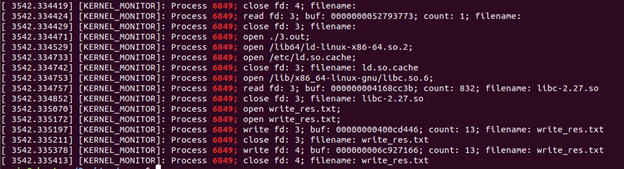
\includegraphics[width = 0.7 \textwidth]{lab_03_3out.png}
        \caption{Пример работы загружаемого модуля ядра.}
        \label{3out}
    \end{figure}

\section{Вывод}
    В данном разделе был обоснован выбор языка программирования, 
    рассмотрены листинги реализованных функций. 
    Приведены результаты работы ПО.

\pagebreak